\documentclass[tikz]{standalone}

\usetikzlibrary{shapes, decorations, arrows ,calc, arrows.meta,
                fit, positioning, automata, shapes.geometric, patterns}

\usepackage{tikz}

\begin{document}

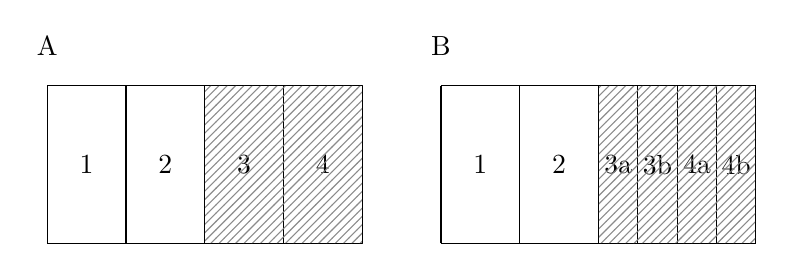
\begin{tikzpicture}
\node[] at (-1, 1.5) {A};nonumber
\node[] at (-0.5, 0) {1};
\node[] at (0.5, 0) {2};
\node[] at (1.5, 0) {3};
\node[] at (2.5, 0) {4};
\draw (-1,1) -- (3,1);
\draw (-1,-1) -- (3,-1);
\draw (-1,-1) -- (-1,1);
\draw (0,-1) -- (0,1);
\draw (1,-1) -- (1,1);
\draw (2,-1) -- (2,1);
\draw (3,-1) -- (3,1);
\filldraw[pattern color=gray, pattern=north east lines, opacity=0.9] (1,-1) -- (1,1) -- (3,1) -- (3,-1) -- cycle;

\node[] at (4, 1.5) {B};nonumber
\node[] at (4.5, 0) {1};
\node[] at (5.5, 0) {2};
\node[] at (6.25, 0) {3a};
\node[] at (6.75, 0) {3b};
\node[] at (7.25, 0) {4a};
\node[] at (7.75, 0) {4b};
\draw (4,1) -- (8,1);
\draw (4,-1) -- (8,-1);
\draw (4,-1) -- (4,1);
\draw (5,-1) -- (5,1);
\draw (6,-1) -- (6,1);
\draw (7,-1) -- (7,1);
\draw (8,-1) -- (8,1);

% Additional lines down
\draw (6.5,-1) -- (6.5,1);
\draw (7.5,-1) -- (7.5,1);

% Shading
\filldraw[pattern color=gray, pattern=north east lines, opacity=0.9] (6,-1) -- (6,1) -- (8,1) -- (8,-1) -- cycle;

\end{tikzpicture}

\end{document}